\section{Evaluation}

This section will explain how Haskell evaluates its expressions and is fundamental to understanding how the language operates.

In summary, Haskell employs \textit{lazy evaluation} which uses \textit{outermost reduction} and \textit{sharing}.

\subsection{Lazy Evaluation}
Haskell is lazy. This means that it will only evaluate an expression when that expression is required; otherwise, the expression is stored in an un-evaluated form as a \textit{thunk}.

An un-evaluated expression may be viewed in GHCi using \texttt{:sprint <expr>}. Underscores represent thunks which have not been evaluated.

To evaluate an expression, Haskell recursively reduces terms and applies atomic calculations where necessary (operations such as \texttt{+} and \texttt{*}).

\subsection{Reduction}
This is how Haskell evaluates expressions.

Anything that appears on the left-hand side of \texttt{=} may be replaced by its right-hand side (and vice versa). Pattern matching is used in more complex replacements. An expression is fully evaluated when it can cannot be further reduced i.e. a value.

\textbf{Example}:
\begin{lstlisting}[language=haskell]
square :: Int -> Int
square x = x * x

f :: Int -> Int -> Int
f x y = y + square x

155 + f 94 10           -- Apply definition of 'f'
= 155 + 10 + square 94  -- Apply definition of 'square'
= 155 + 10 + 94 * 94    -- Atomic operation '(*)'
= 155 + 10 + 8836       -- Atomic operation '(+)'
= 155 + 8846            -- Atomic operation '(+)'
= 9001                  -- Fully evaluated
\end{lstlisting}

As Haskell functions are mathematically pure, the order of reduction does not matter- the end result is the same. We could reduce \texttt{155 + 10} before applying \texttt{square} and the result would still be the same.
This is known as the \textit{Church-Rosser} theorem and applies to some variants of lambda-calculus.

There are two reduction variants.

\subsubsection{Innermost Reduction}
Fully evaluate the arguments of a function \textit{before} the function definition is applied.

\begin{lstlisting}[language=haskell]
fst (square 3, square 4)
= fst (3*3, square 4)   -- Apply 'square'
= fst (9, square 4)     -- Atomic operation '(*)'
= fst (9, 4*4)          -- Apply 'square'
= fst (9, 16)           -- Atomic operation '(*)
= 9                     -- Apply 'fst'
\end{lstlisting}

\subsubsection{Outermost Reduction}
Fully apply function definitions first.

\begin{lstlisting}[language=haskell]
fst (square 3, square 4)
= square 3               -- Apply 'fst'
= 3*3                    -- Apply 'square'
= 9                      -- Atomic operation '(*)'
\end{lstlisting}

\subsubsection{Graph Reduction}
Under the hood, Haskell uses graph reduction to evaluate expressions. Essentially, every expression which is defined is part of a large graph structure. Vertices contains either a function which can be reduced, or an atomic value.

\medskip
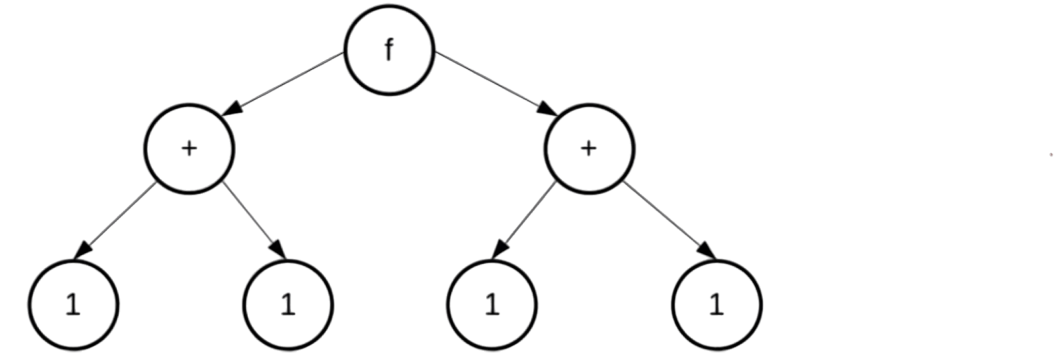
\includegraphics[width=0.5\textwidth]{latex/assets/graph-reduction.png}

To implement the concept of ``sharing'', each non-value vertex points to a placeholder vertex where the resulting value will be stored, which in turn points to the expression. Therefore, sharing is where two or more placeholder vertices point to the same expression.

\medskip
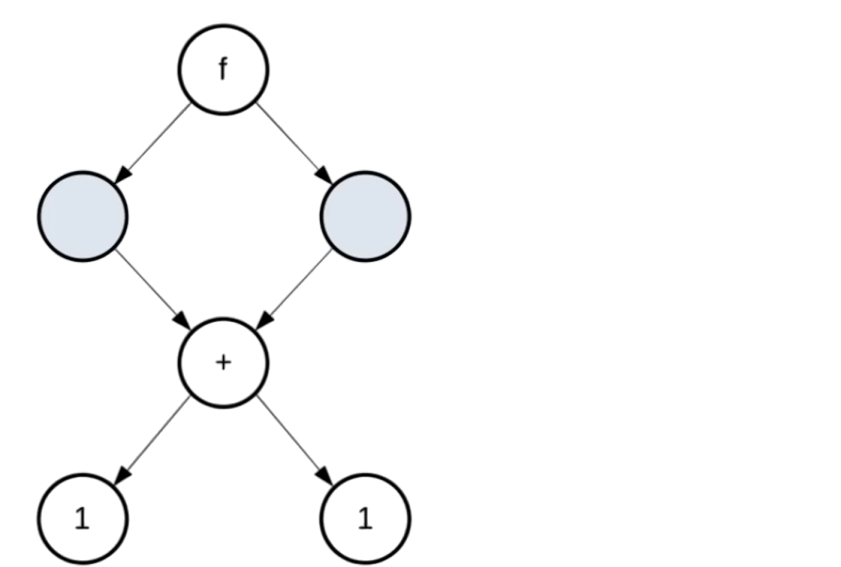
\includegraphics[width=0.5\textwidth]{latex/assets/graph-reduction-sharing.png}

\subsection{Sharing}
Possible due to lack of side effects, thunks which are equivalent need only be evaluated once and its value shared.
This is done by memoising evaluated thunks to avoid re-evaluation of equivalent thunks in the future.

\begin{lstlisting}[language=haskell]
(1 + 1) + 2 + (1 + 1)
= (2) + 2 + (2)
= (2) + 4
= 6
\end{lstlisting}

\subsection{Normal Form}
An expression is in a normal form if and only if it is fully evaluated (i.e. no further reductions can be applied).

Examples:
\begin{lstlisting}[language=haskell]
1 + 1 => 2
(1, 2+2) => (1, 4)
[True && False] => [False]
(\x -> x * 10) -- Already in normal form!
\end{lstlisting}

Note that the following are not in normal form:
\begin{itemize}
  \item \textit{Function definitions}. Expand the definition into a value.
  \begin{lstlisting}[language=haskell]
f x = ...
-- Becomes
f = \x -> ...\end{lstlisting}
  \item \textit{Top-level pattern matching}. Expand into a \texttt{case .. of ..} expression.
  \begin{lstlisting}[language=haskell]
f <p1> = <e1>
f <p2> = <e1>
-- Becomes
f = \x -> case x of
    p1 -> e1
    p2 -> e2
\end{lstlisting}
\end{itemize}

\subsubsection{Weak Head Normal Form}
An expression which is fully evaluated \textit{up to \textbf{at least}} the first data constructor. Values/equations in WHNF are:-
\begin{enumerate}
  \item Data constructors
  \item Built-in functions applied to too few arguments e.g. \texttt{(+ 2)}
  \item Lambda expressions
\end{enumerate}

\begin{lstlisting}[language=haskell]
1 + 1 => 2
(1, 2+2) -- In WHNF as values are inside a data constructor
[True && False] => _ : _ -- The values do not matter. Only the constructor '(:)' matters in WHNF.
\end{lstlisting}

The \texttt{seq} function is \textit{strict} in its first argument - it enforces its first argument to be evaluated to WHNF. This function is defined this way explicitly in GHC and is one of the only functions to do this.